
    %\ifx\isEmbedded\undefined
%	% Loading common settings
%	\input{macros/common}
%	% Loading common variable definitions 
%	\input{macros/macros}
%	\begin{document} 
%\else
%\fi
%

%\setcounter{chapter}{33}
\chapter{Object recognition}

why we need a learning based system?

Output representation (this can  just  be a figure): this addresses the question of how is the output specified (a label, a bounding box, a 3D model, ...).
		There  are many tasks that researchers use to address  the problem of recognition. Although  the ultimate goal is to tell what something it is by looking at it, the way that you will answer the question will change the approach that you will  use. For instance, you could say "that is a chair" and just point  at it, or I could ask you to indicate all of the visible parts of the chair, which might be a lot  harder if the chair is partially occluded by other chairs producing a sea of legs. It could be hard to precisely delineate the chair if we can not tell which legs belong to it. 
		
		FIGURE: show an image where the chair is clearly visible, and another with a chair in a busy  scene. 
		Maybe  the rest could be: function and loss
		image classification (is the object present somewhere?)
		localization: bounding boxes
		semantic segmentations: pixel labeling 
		panoptic segmentation: segments and instances
		instance identification (my chair vs a chair)
		objects, parts, attributes, stuff
		


Following blocks
\begin{itemize}
\item Task specification
\item Representation
\item Features
\item Classifier
\end{itemize}


\begin{figure}[h]
    \centering
    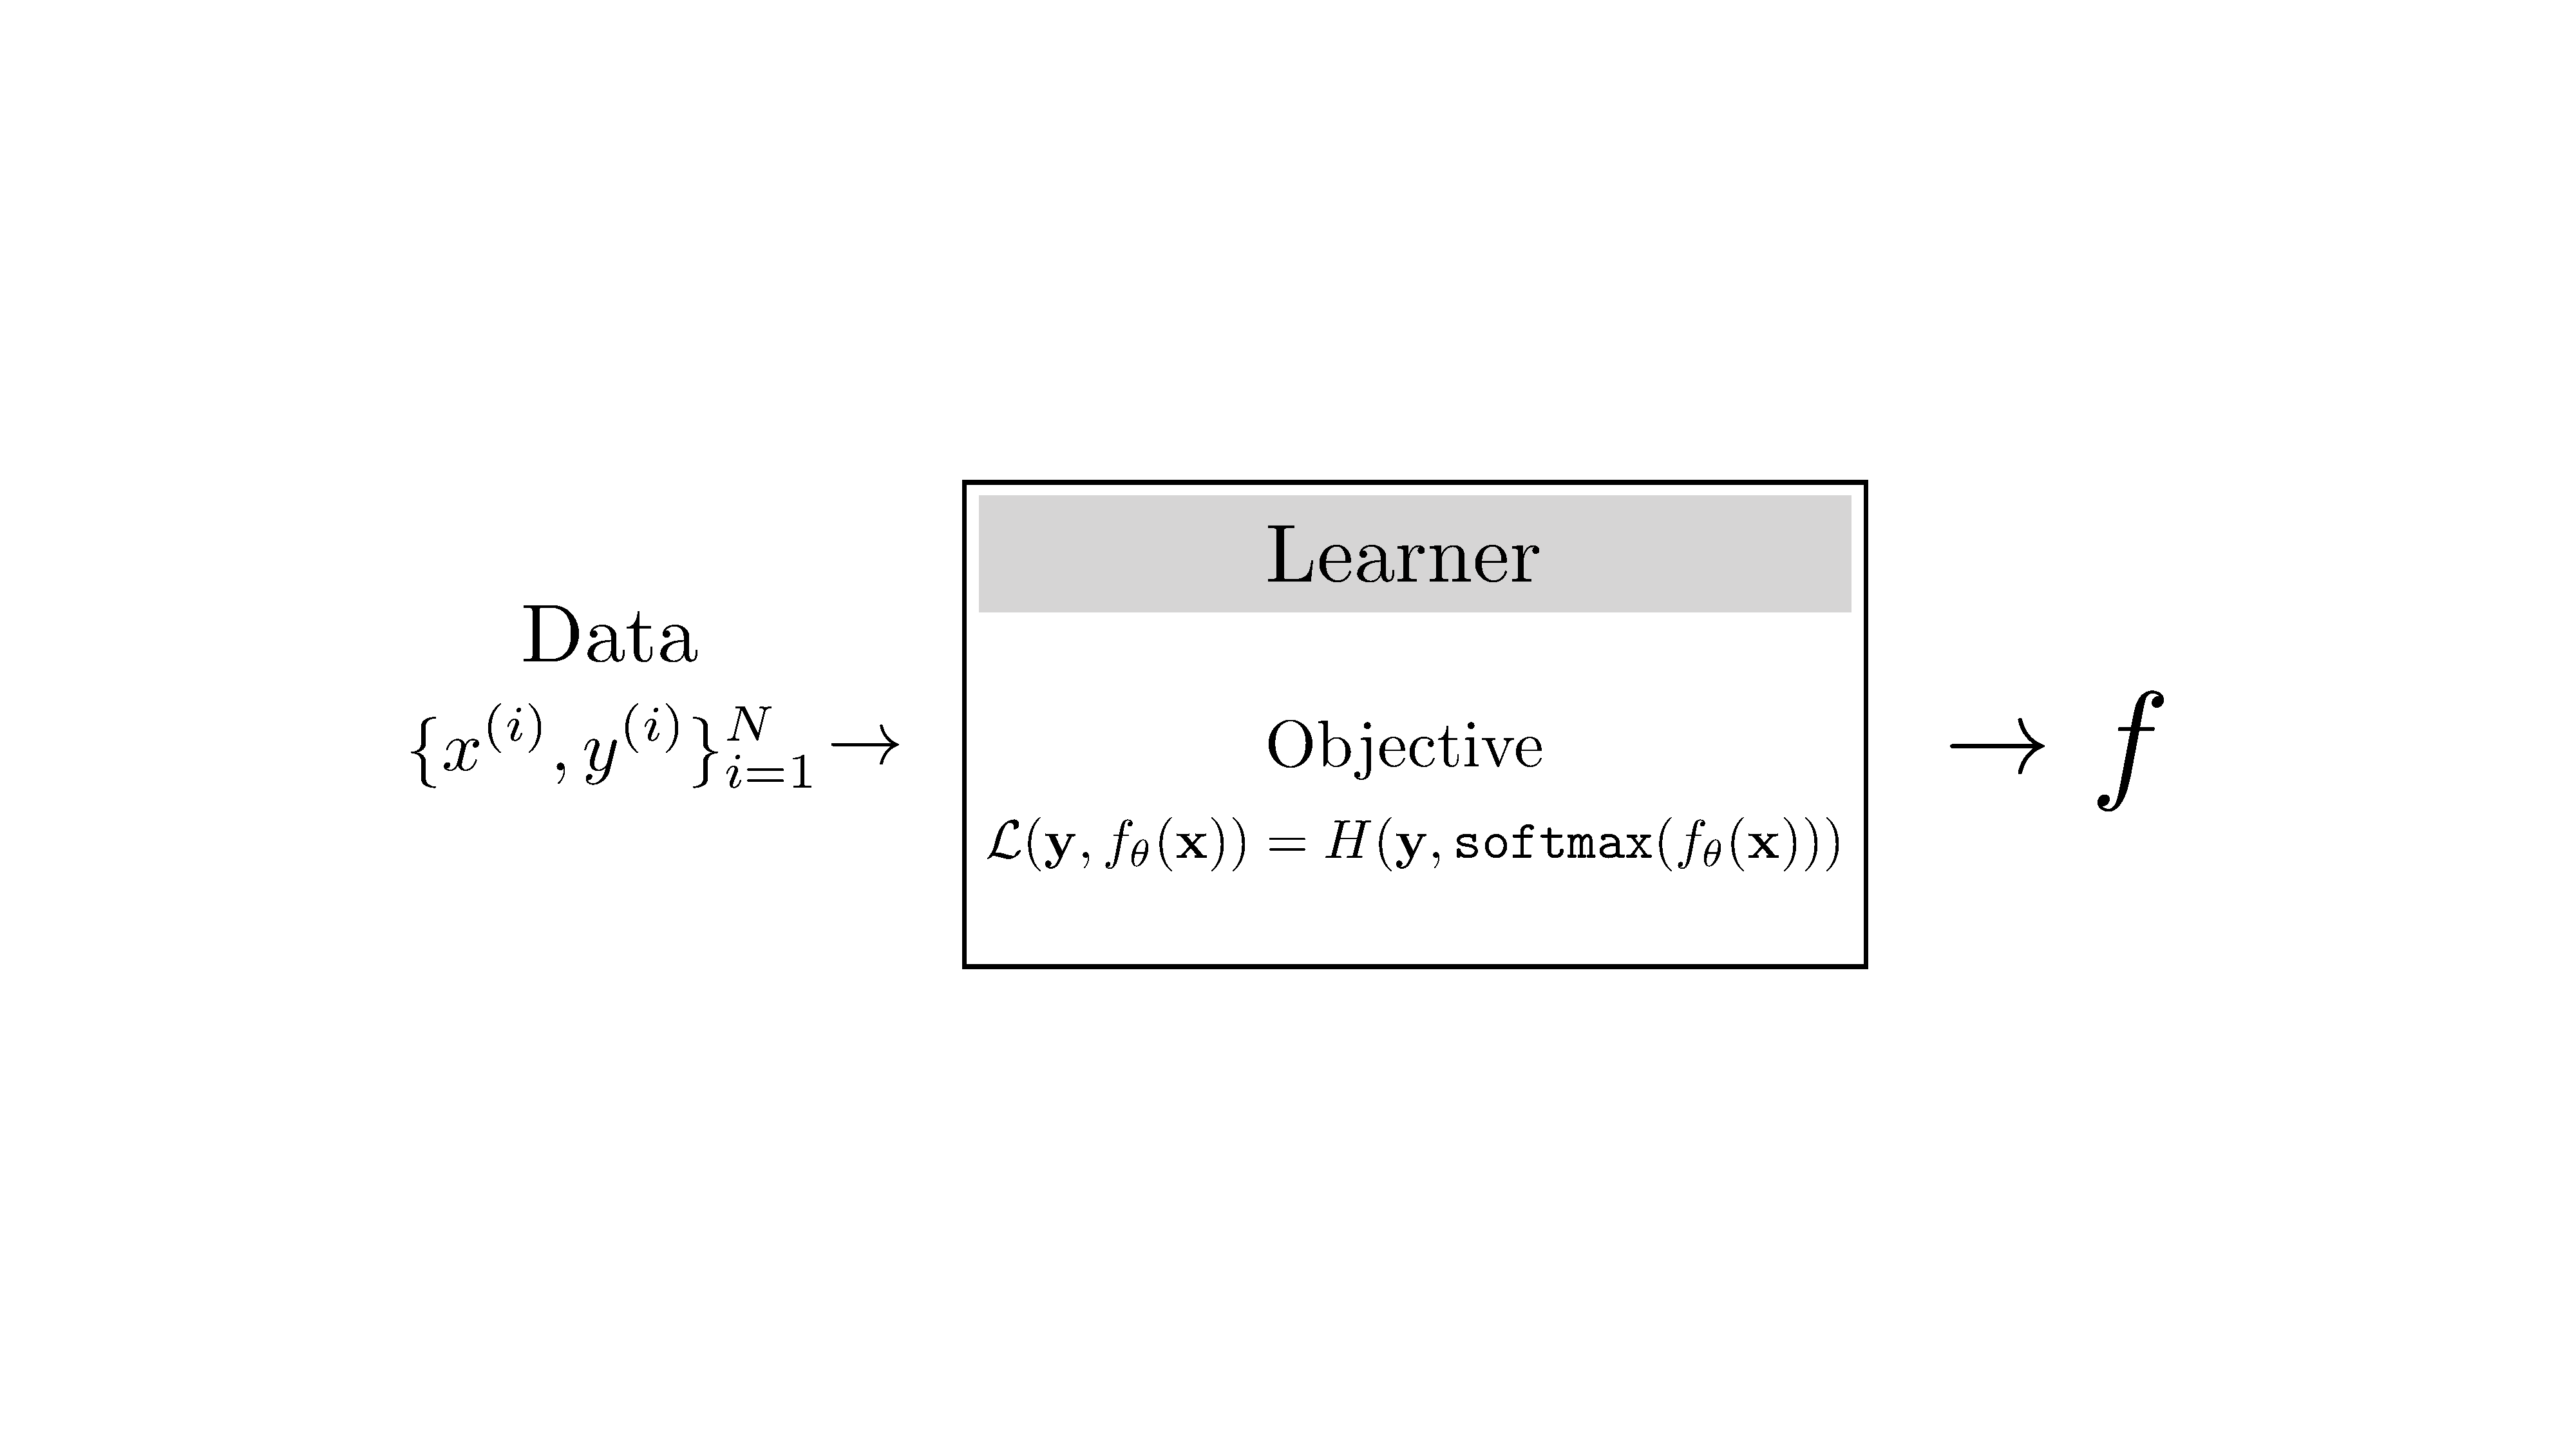
\includegraphics[width=0.7\linewidth]{./figures/intro_to_learning/softmax_regression_learning_problem.pdf}
    \label{fig:softmax_regression_learning_problem}
\end{figure}


Why is object recognition a hard problem? Objects 

Intrinsic changes:
\begin{itemize}
    \item Changes in viewpoint
    \item Changes in scale
    \item Changes in style and appearance
\end{itemize}

Extrinsic changes:
\begin{itemize}
    \item Changes in illumination
    \item Complex background, which similar statistics than the objects themselves. Objects are made of edges, textures, just like the background is. Objects are rarely in front of a flat background. 
    \item Occlusions
\end{itemize}

Objects live in a 3D world, but we only observe 2D images of them.

\section{Image classification}

%\subsection{Definition}

Image classification is one of the simplest tasks in object recognition. The goal is to answer the following question:

\centerline{
{\bf Is object class $c$ present anywhere in the image $\bf x$?}
}

It assumes that there is a closed vocabulary of object classes. For instance, if our vocabulary contains $K$ classes, we can loop over the classes ask the same question for each class. This task does not try to localize the object in the image, or to count how many instances of the object are present.
 
\subsection{Formulation}

One canonical task in object recognition is to build a function $f$ that takes as input image $\bf x$? and answers the following question: {\bf is object class $c$ present anywhere in the image $\bf x$?} The output, $\hat {\bf y}$, of the function will be a binary response: $1=yes$ and $0=no$. 
%We can answer this question in a mathematical form by building a function that maps the input image ${\bf x}$ into an output vector $\hat {\bf y}$:
\begin{equation}
\hat {\bf y} = f({\bf x})
\end{equation}

In general we want to classify an image according to multiple classes. We can do that by having as output a vector $\hat {\bf y}$ of length $K$, where $K$ is the number of classes. Component $c$ of the vector $\hat {\bf y}$ will indicate whether class $c$ is present or absent in the image. For instance, the training set will be composed of examples of images and the corresponding class indicator vectors as shown in the following image (here for $K=3$):

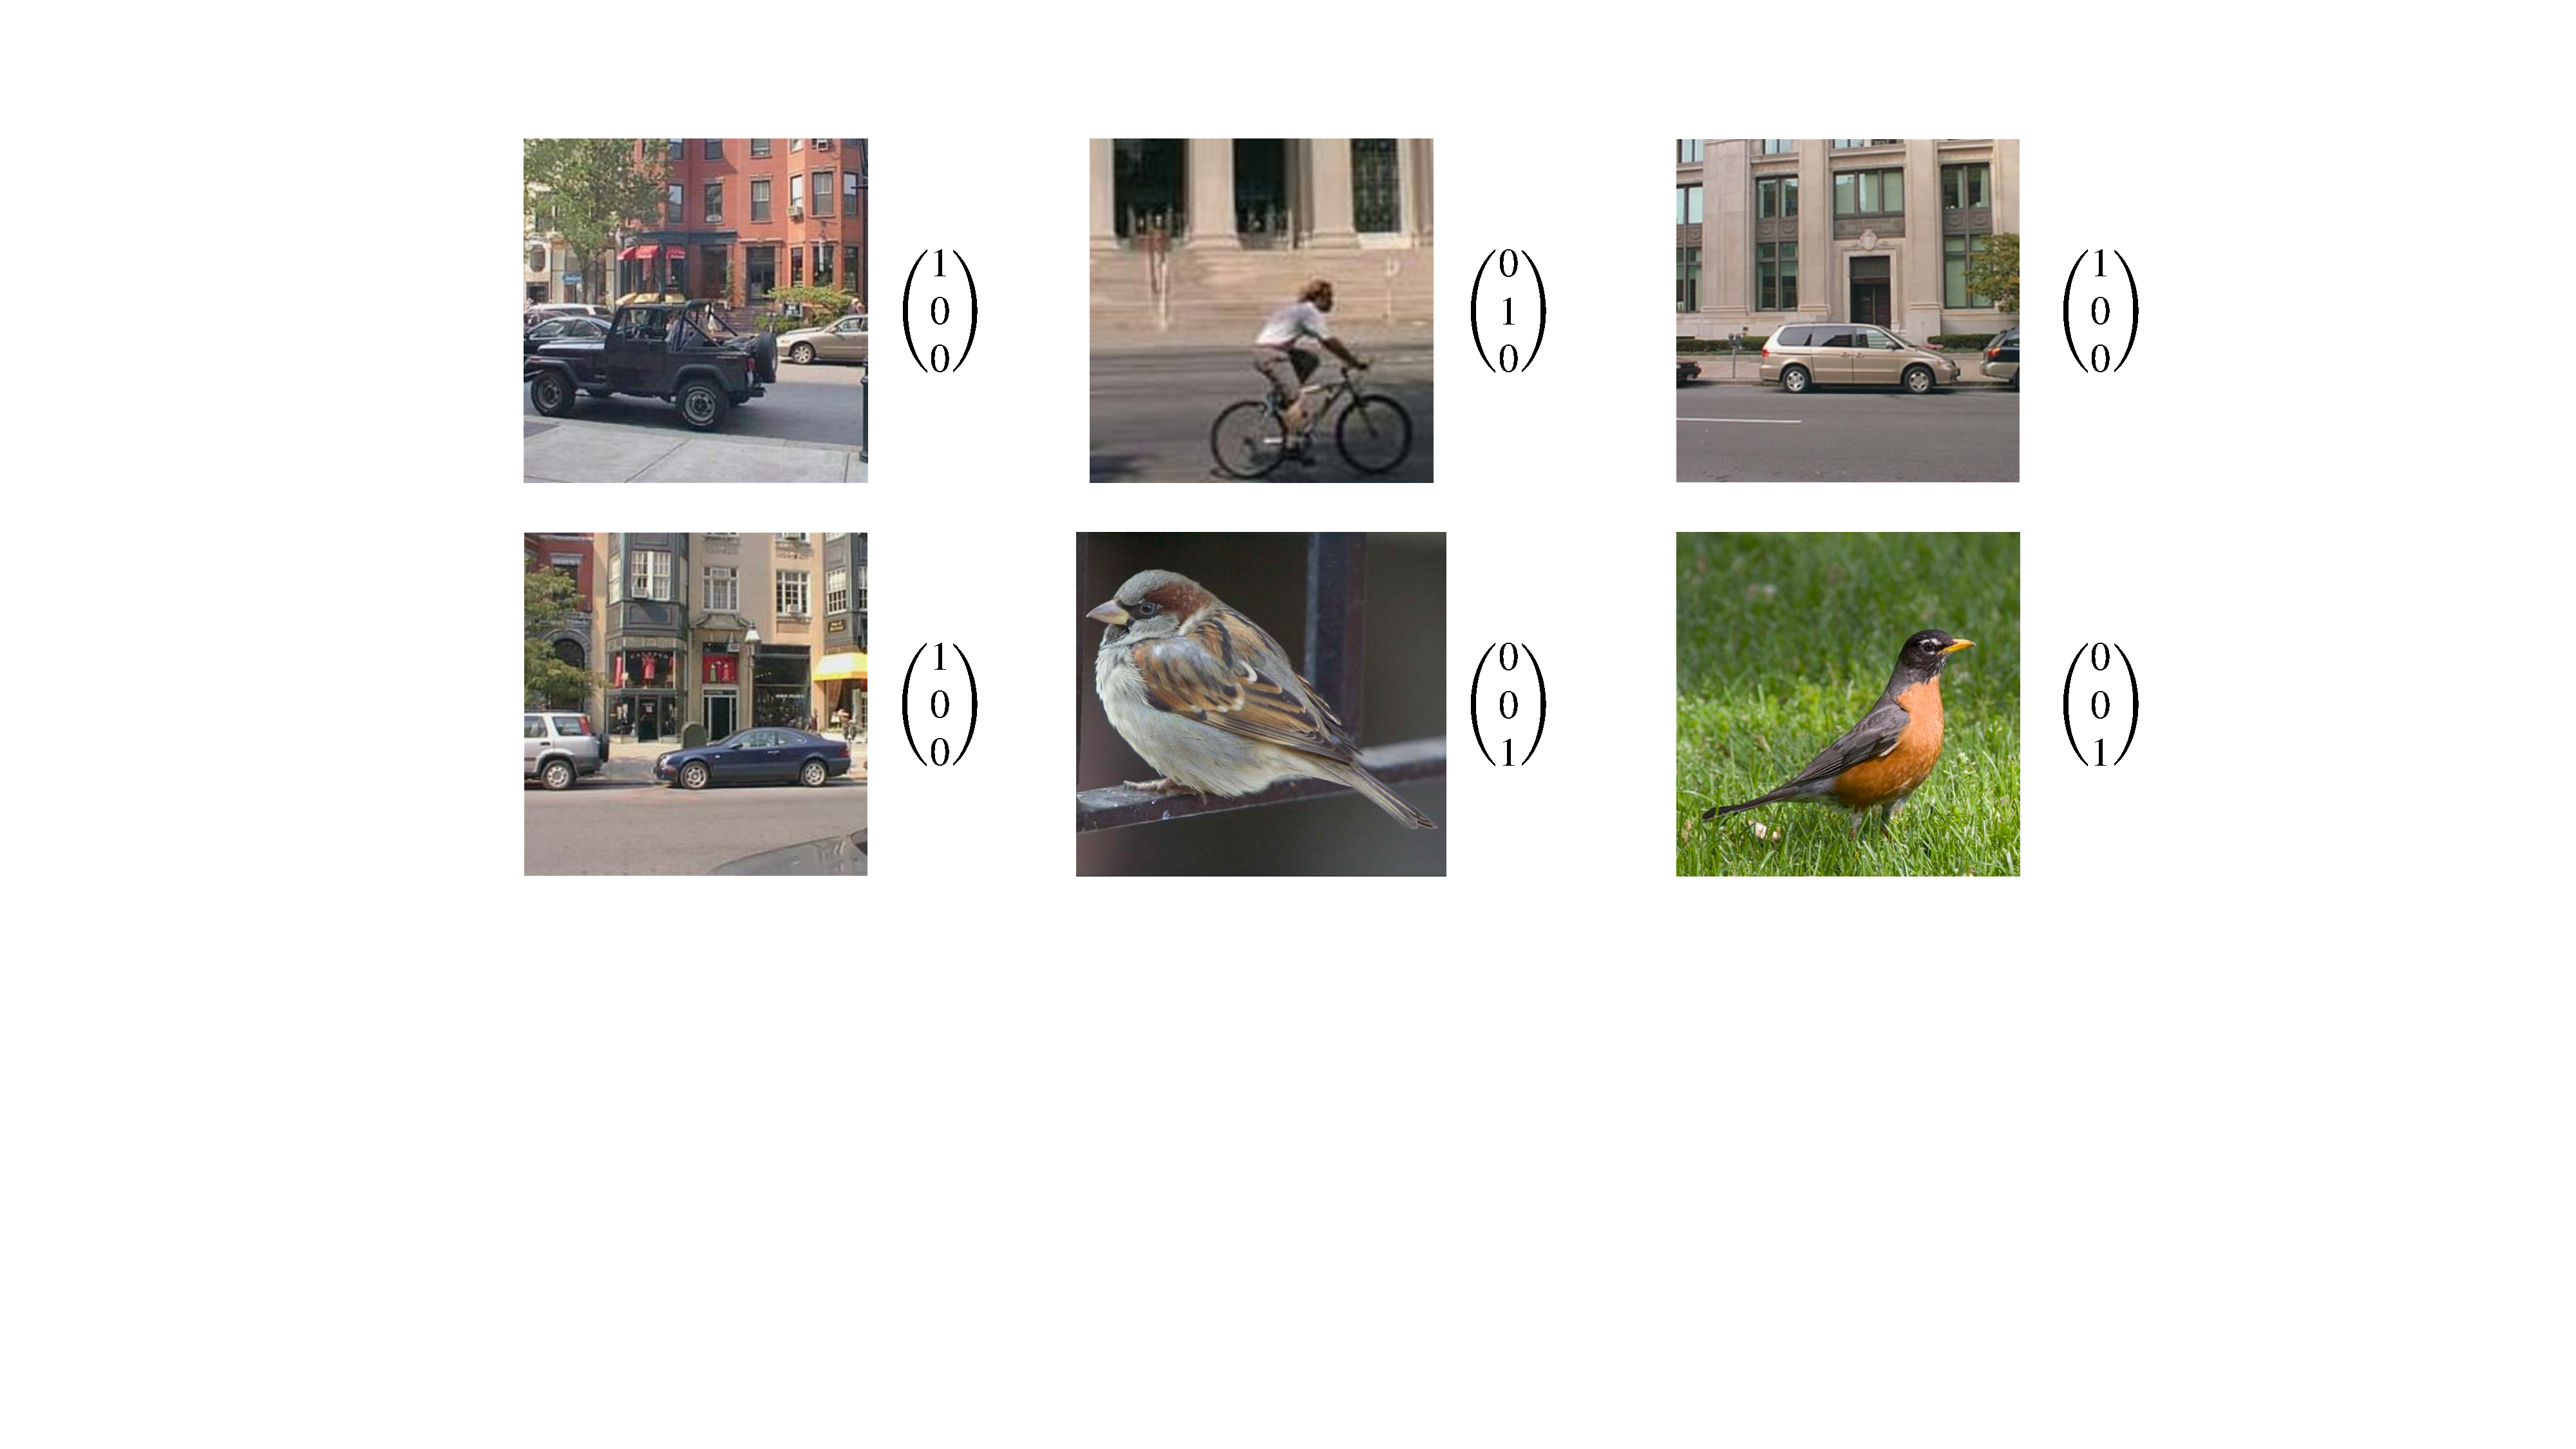
\includegraphics[width=1\linewidth]{figures/object_recognition/classification_training_set.pdf}

We want to enrich the output so that it also represents the uncertainty in the presence of the object. This uncertainty can be the result of a function $f$ that does not work very well, or from a noisy or blurry input image $\mathbf{x}$ where the object is difficult to see. One can formulate this as computing the function $f$ that takes as input the image ${\bf x}$ and outputs the probability distribution of the $K$ classes: $\hat{\mathbf{y}}=(y_1, y_2, ..., y_K)$, where $y_c$ is the probability that object class $c$ is present in the image $\mathbf{x}$. 

One common assumption is that only one class, among the $K$ possible classes, is present in the image, which results in the following constraint: 
\begin{equation}
\sum_{c=1}^K y_c=1
\end{equation}
and $0>y_c>1$.
In the toy example above with three classes, the valid solution for $\mathbf{y}=(y_1, y_2, y_3)$ is constrained to lie within the triangle (simplex) in the figure bellow:

\marginnote{Simplex:
\centerline{
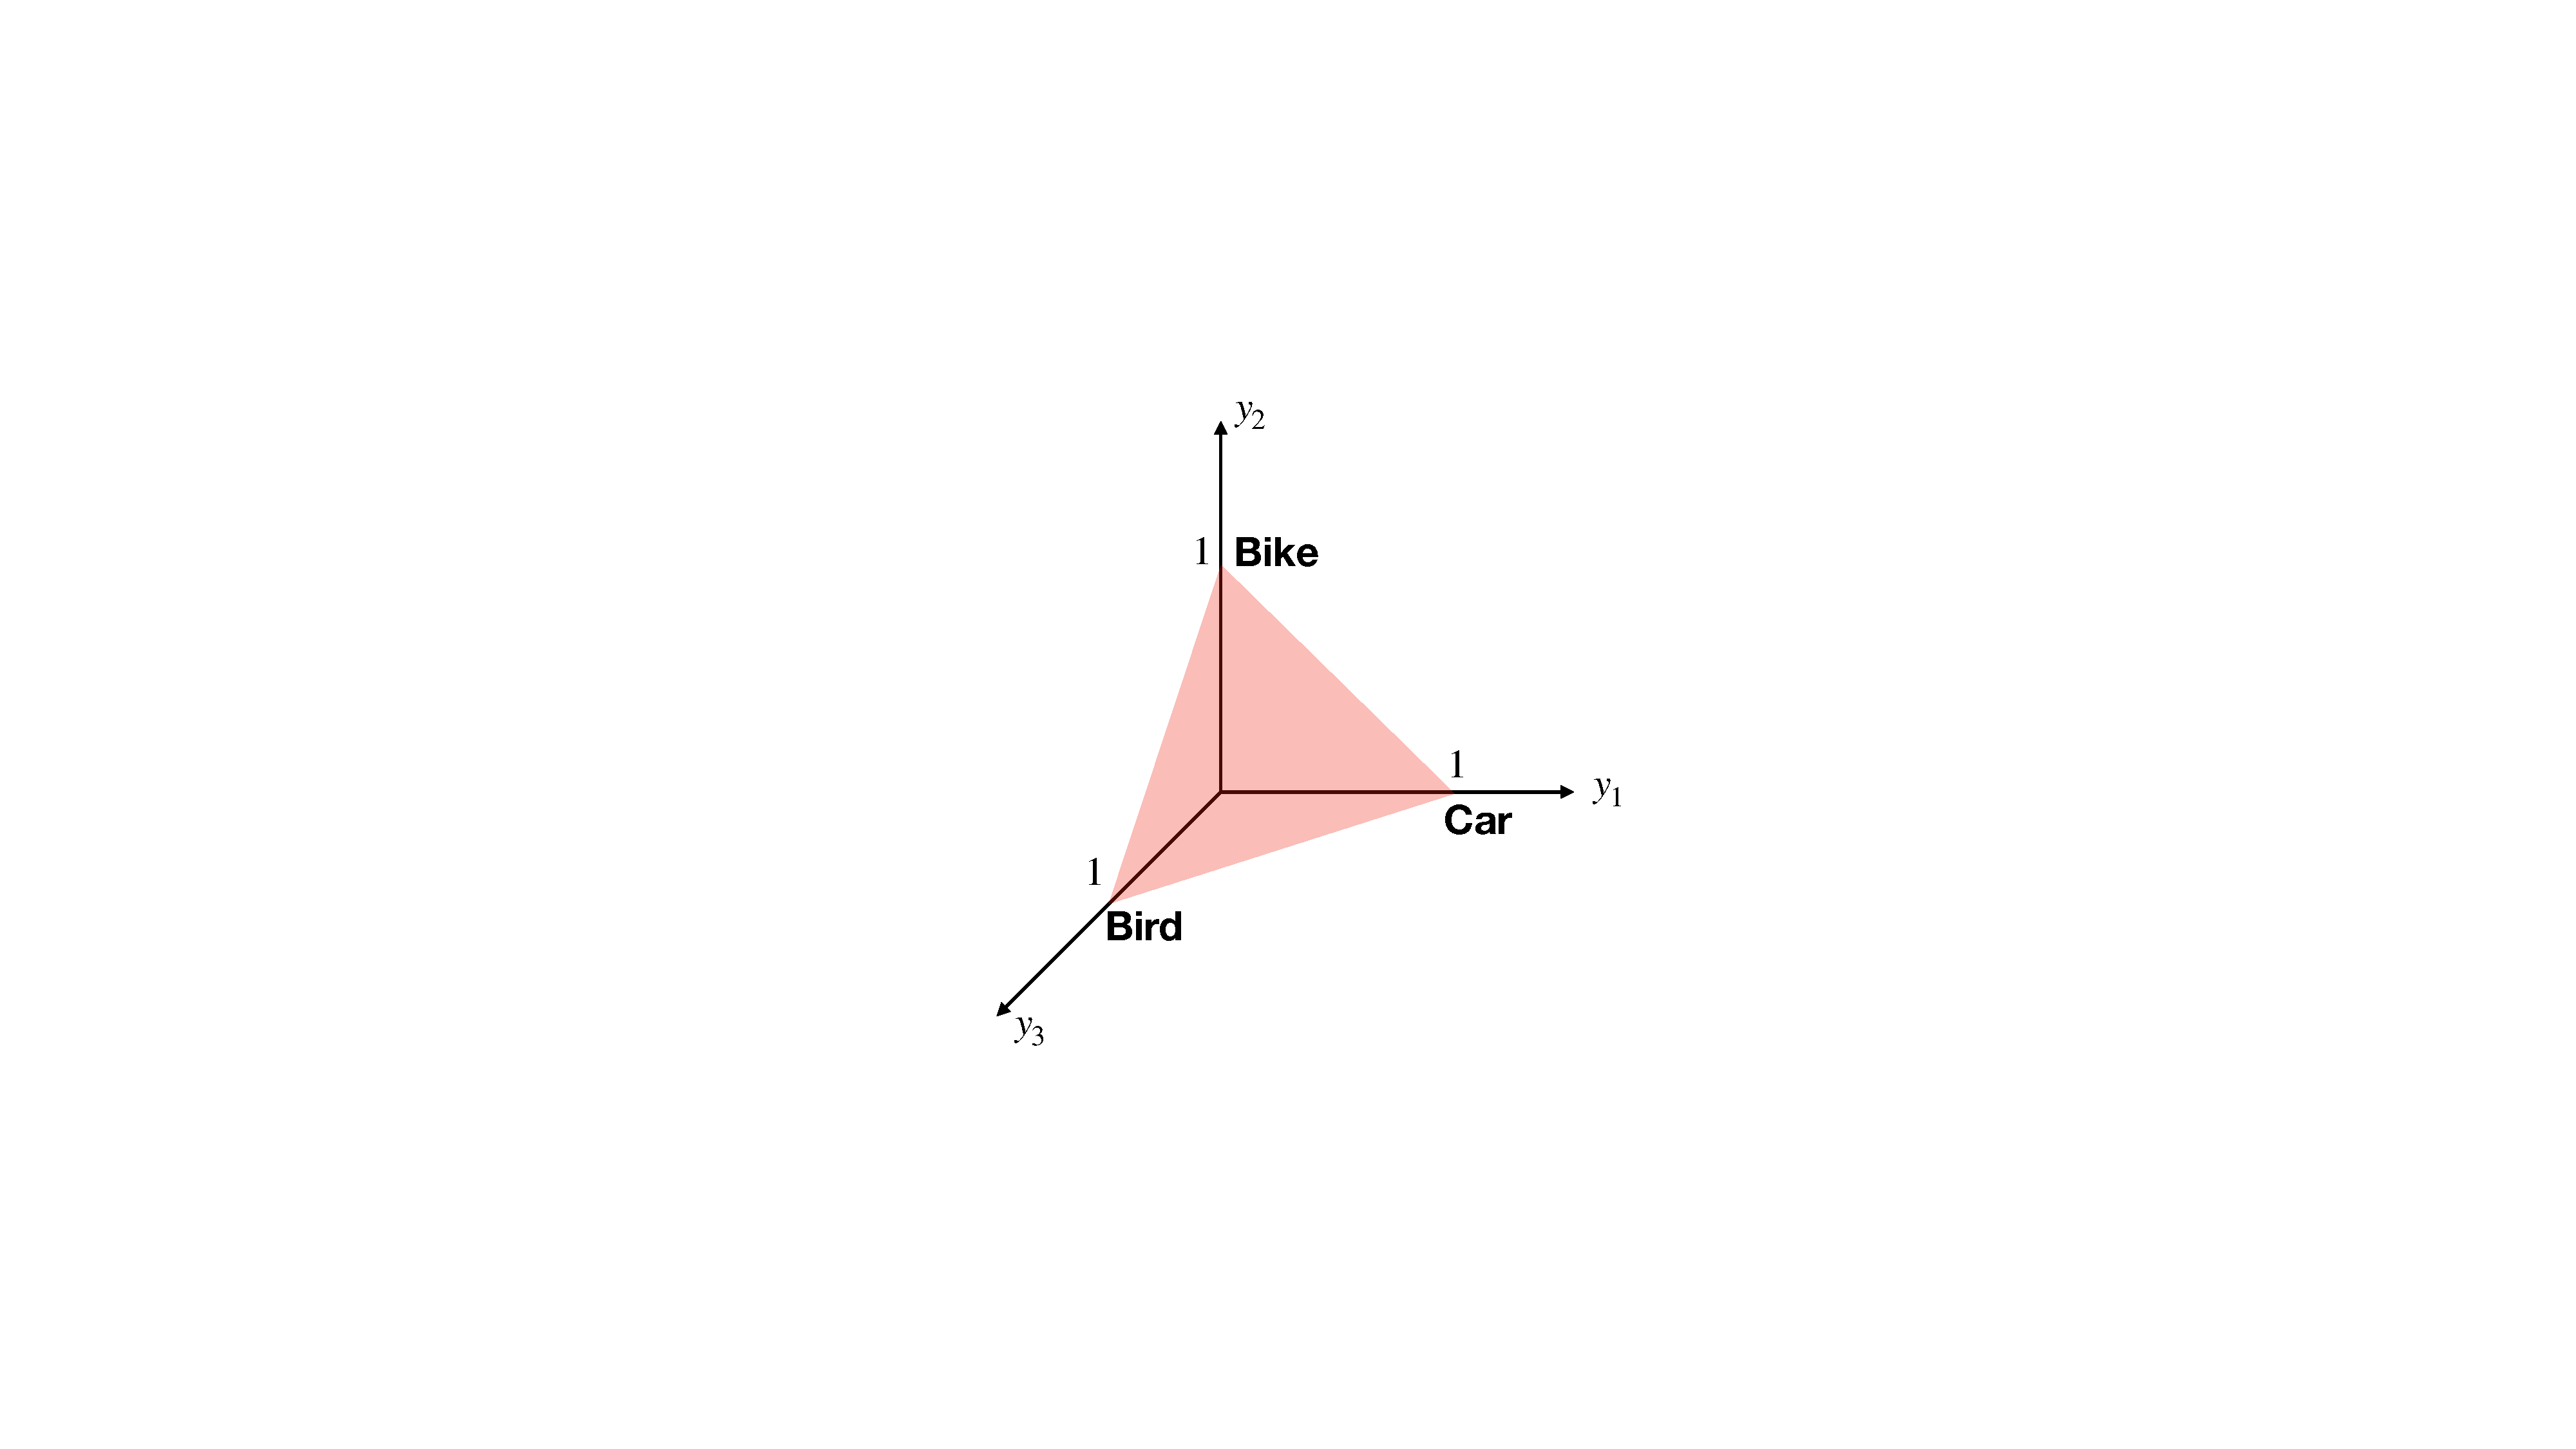
\includegraphics[width=1\linewidth]{figures/object_recognition/simplex.pdf}
}
}

Under this formulation, the function $f$ is a mapping $f:\mathbb{R}^{nm3} \rightarrow S^K$ from the set of RGB images to the simplex of length $K$. 


\subsection{Classification Loss}


\begin{equation}
    \mathcal{L}(\hat{\mathbf{y}},\mathbf{y}) = \mathbbm{1}(\hat{\mathbf{y}}=\mathbf{y}).
\end{equation}


Under this definition, the errors that the function $f$ makes is the number of missplaced ones (i.e., the {\bf miss-classification error}) over the dataset. 

Finding the function $f_\theta$ parameters requires defining a loss function that we will optimize during the training stage. 
%Loss function: 
%The probability of the ground truth data under the output distribution: 
If we interpret the function $f$ as estimating the probability $p({\bf y}_c=1 | {\bf x}, \theta) = \hat {\bf y}_c$. The likelihood of the ground truth data is:
\begin{equation}
\prod_{t=1}^T \prod_{c=1}^K \left( \hat {\bf y}_{c,t} \right) ^{{\bf y}_{c,t}}
\end{equation}

\begin{align}
    \mathcal{L}(\hat{\mathbf{y}},\mathbf{y}) = H(\mathbf{y}, \hat{\mathbf{y}}) = - \sum_{k=1}^K y_k \log \hat{y}_k.
\end{align}

where the first product loops over all $T$ training examples, and the second product loops over all the classes $K$. We want to find the parameters $\theta$ that maximize the likelihood of the ground truth labels for whole training image. As we have seen in chapter XXX, maximizing the likelihood corresponds to minimizing the cross entropy loss:
\begin{equation}
    Loss = - \sum_{t=1}^{T} \sum_{c=1}^{K} y_{c,t} \log (\hat y_{c,t})
\end{equation}

\marginnote{Cross entropy loss: pictorial description of how it works.}

\subsection{Architecture}

The function $f$ is constrained to belong to a set of possible function. For instance, $f$ might belong to the space of all the functions that can be built with a neural network. In such a case the function is specified by the network parameters $\theta: f_\theta$. When using a neural net, the vector $\hat{\mathbf{y}}$ is usually computed as the output of a softmax layer. 

\subsection{Evaluation}

classification performance

Confusion matrix

Precision-recall

\subsection{Shortcomings}


Is it possible to classify an image without localizing the object?

How can we answer to the question "is object c present in the image?" without localizing the object. 

One possibility is that the function $f_\theta$ has learned to localize the object internally but the information about the location is not being recorded in the output. Another possibility is that the function has learned to use other cues present in the image (biases in the dataset).

 As it is no trying to localize an object, the function $f$ will not get penalized if it uses shortcuts such as only recognizing one part of the object (e.g., such as the head of dogs, or car wheels),  make use of contextual biases in the dataset (e.g., all images with grass and blue skies have horses, or all streets have cars) or detect unintended correlations between low-level image properties and the image content (e.g., all images of insects have a blurry background). As a consequence, image classification performance could misslead us into believing that the classifier works well and that it has learned a good representation of the object class it classifies. 

Another shortcoming of this task is that it assumes that we can actually answer the question. But what happens if class definitions are ambiguous or class boundaries are soft? Even in cases were we believe that the boundaries might be well defined, it is east to find images that will challenge our assumption, as shown in fig.~\ref{fig:whatisacar}.


\begin{figure}
\centerline{

\includegraphics[width=0.32\linewidth]{figures/object_recognition/IMG_1260.jpeg}
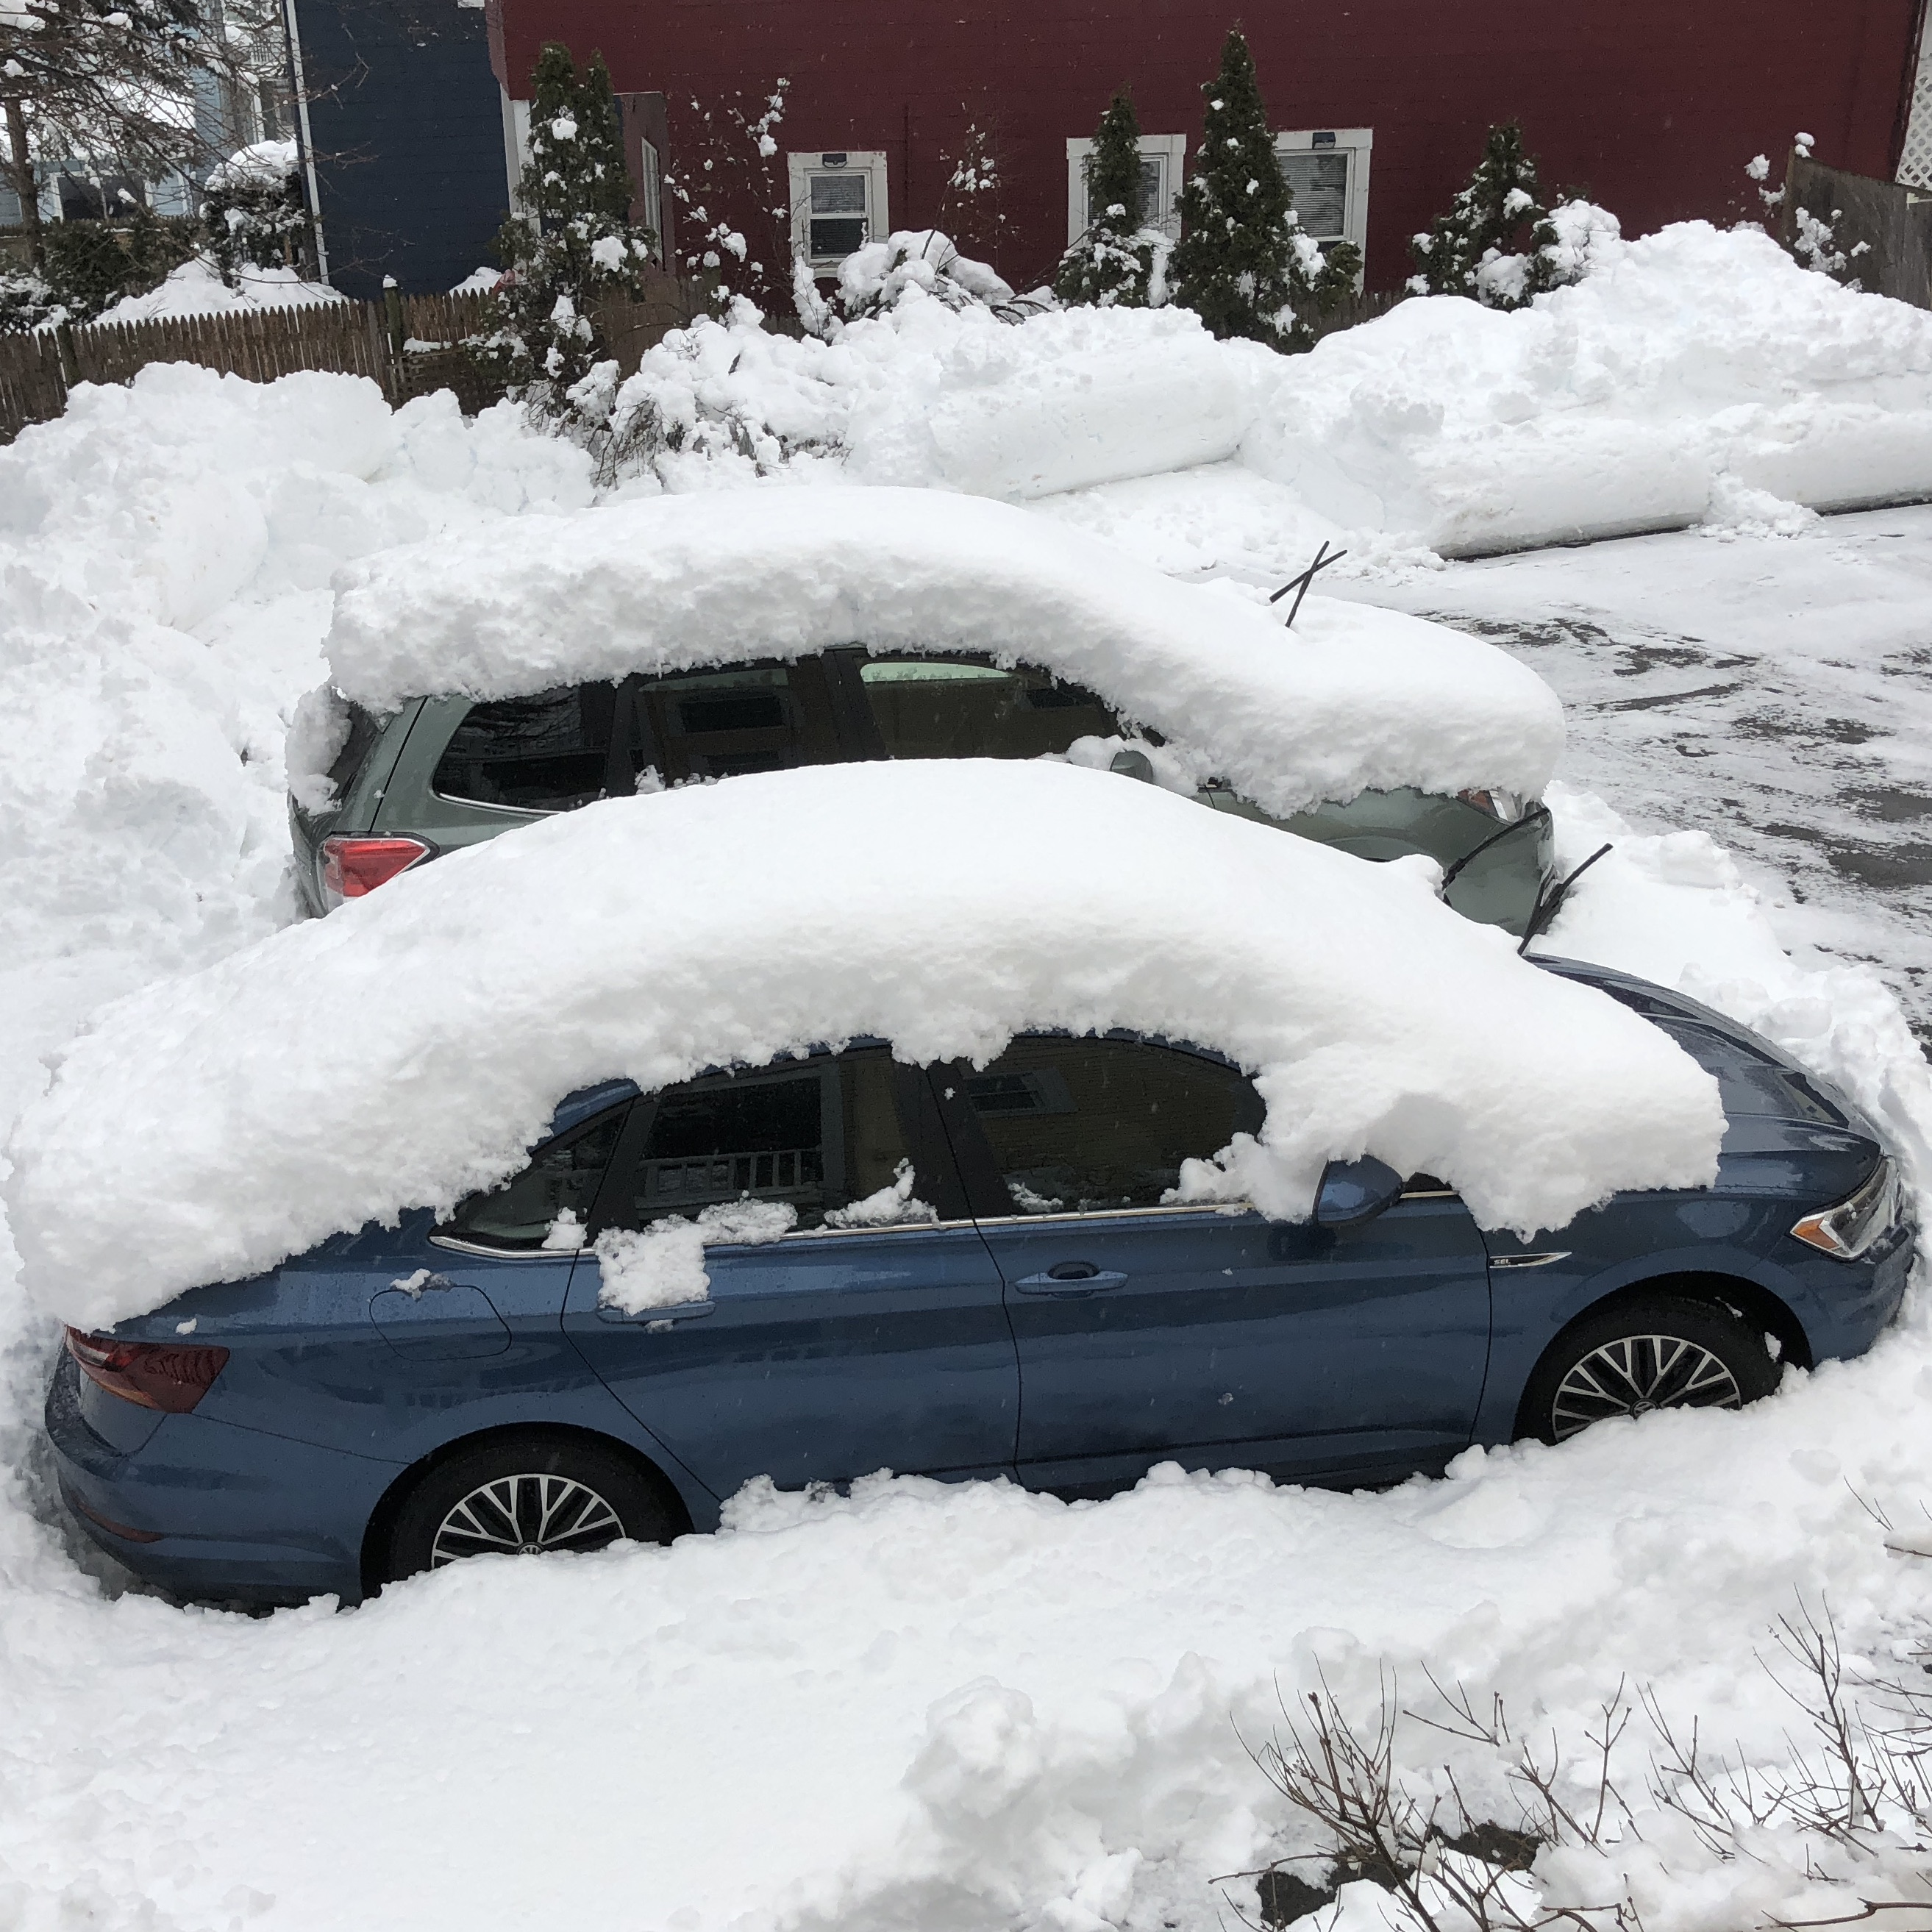
\includegraphics[width=0.32\linewidth]{figures/object_recognition/IMG_7095.jpeg}
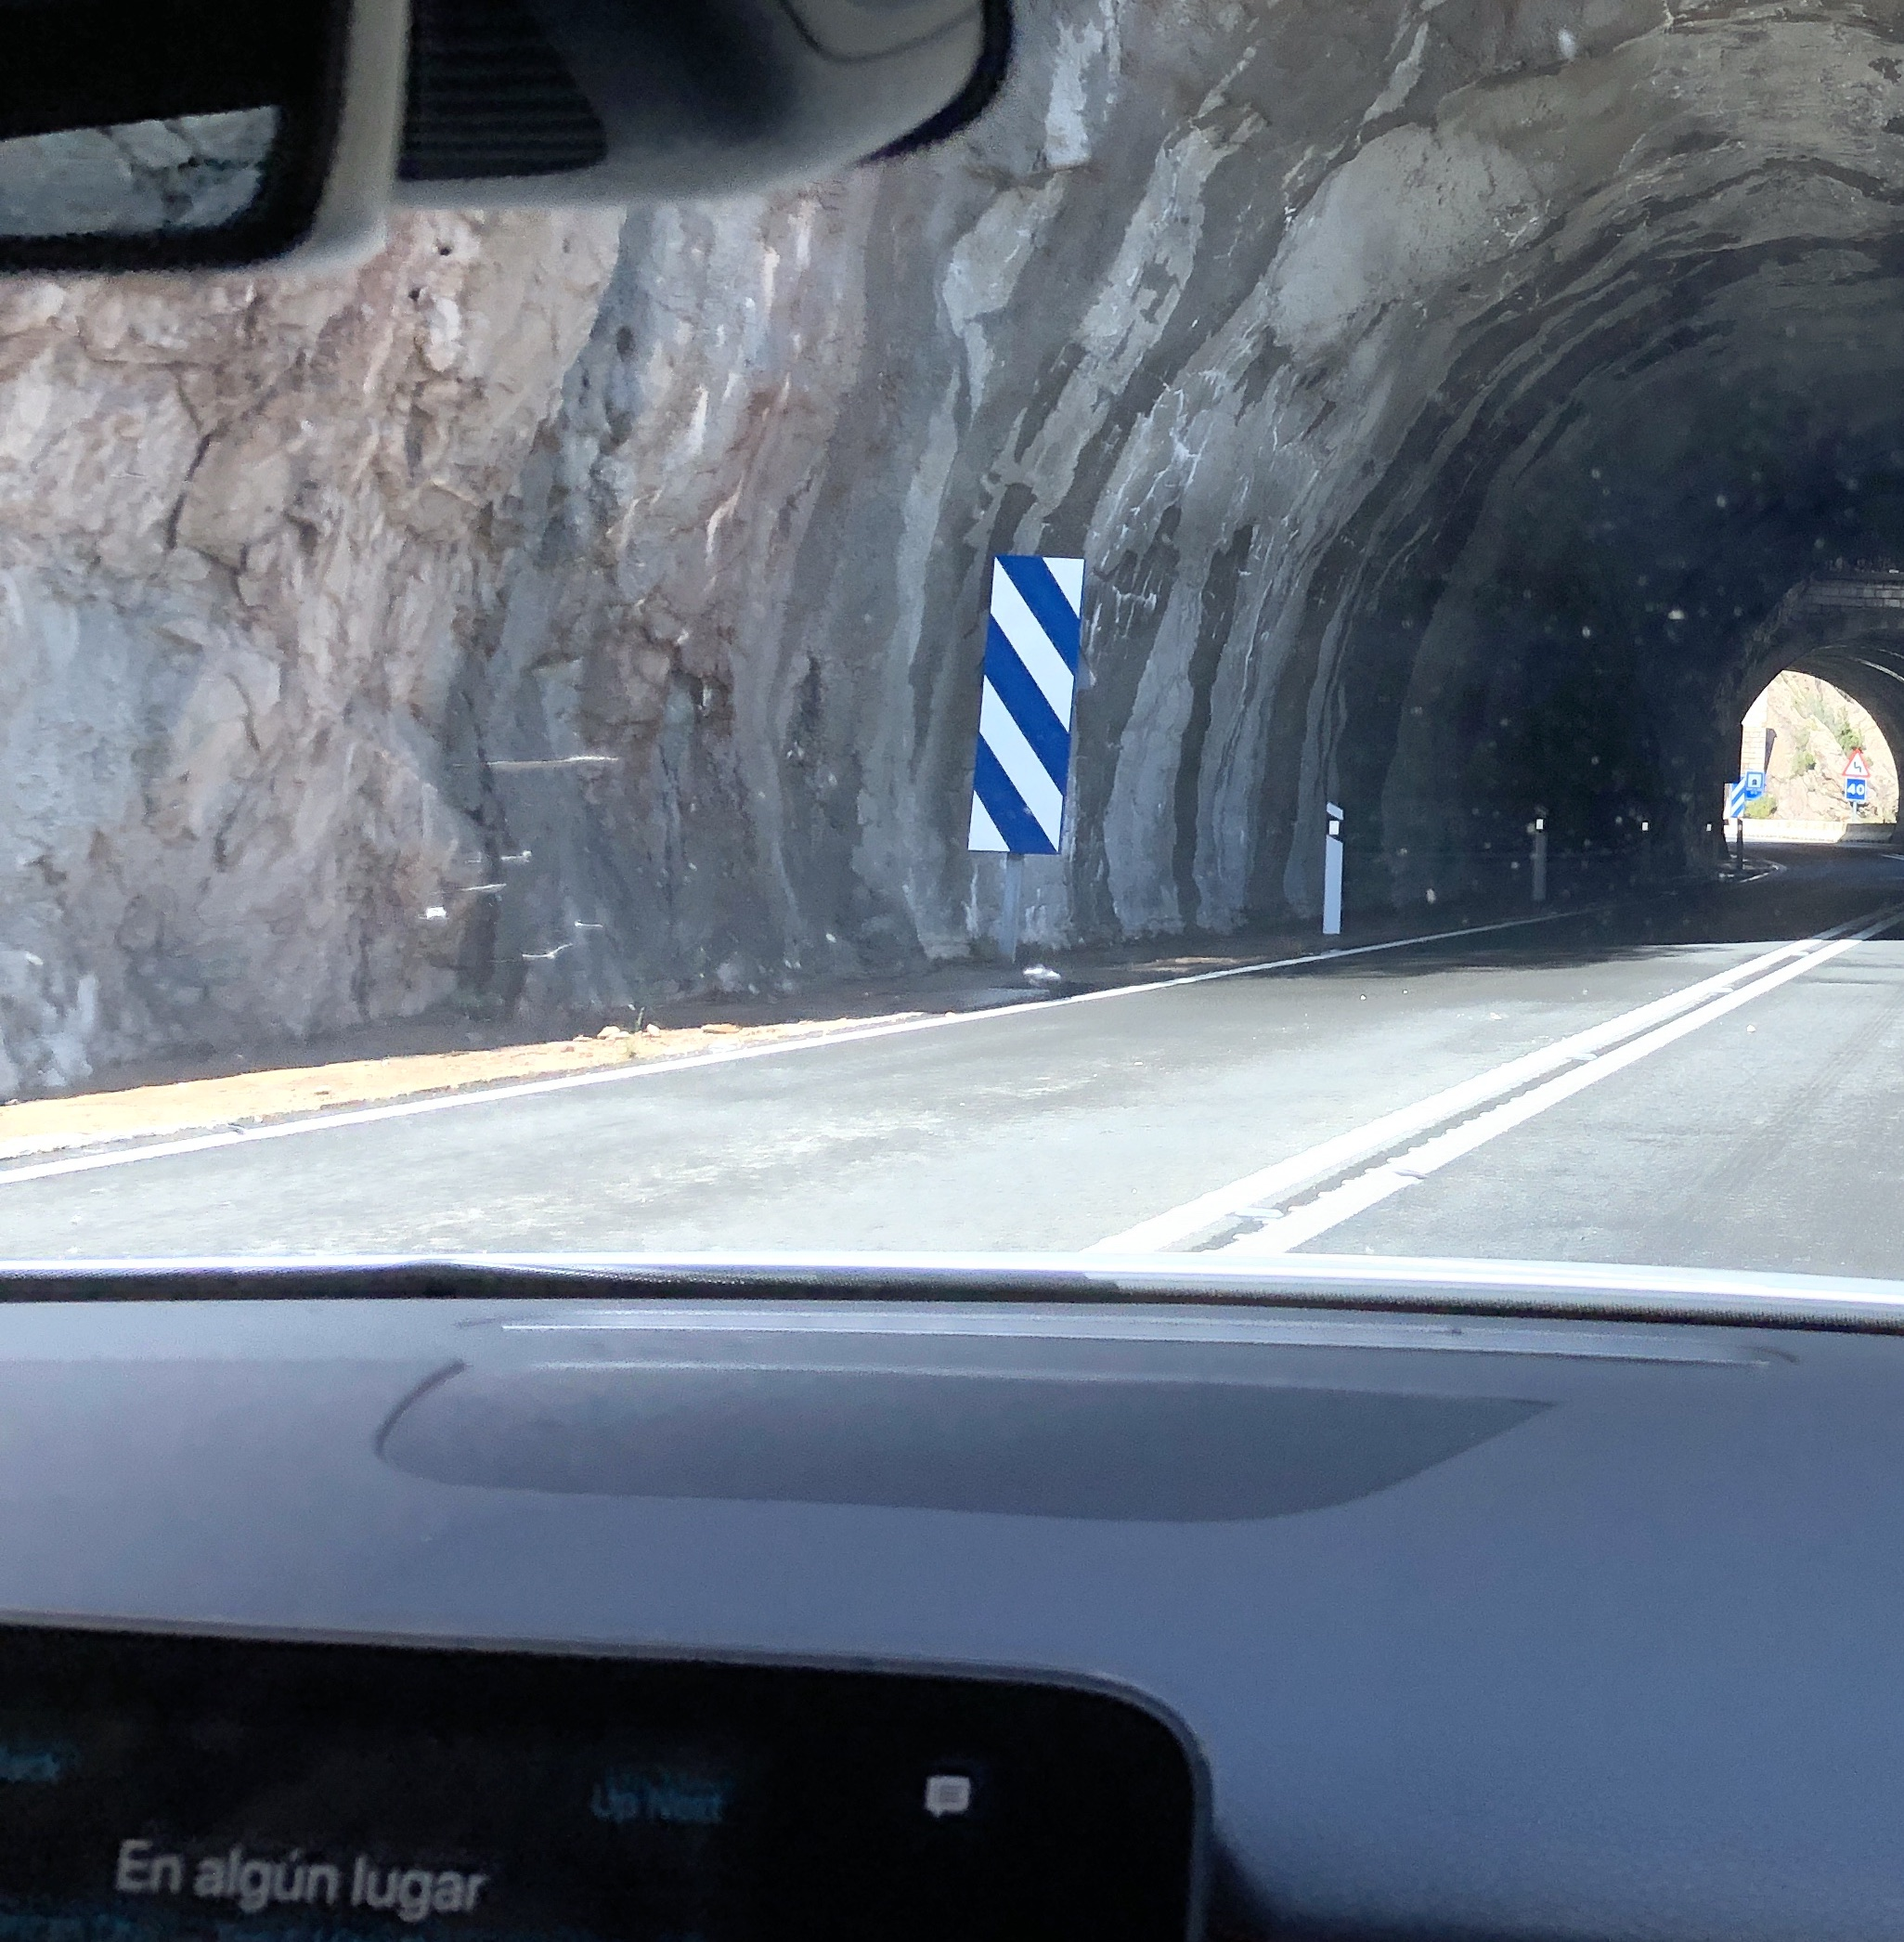
\includegraphics[width=0.32\linewidth]{figures/object_recognition/IMG_9933.jpeg}
}
\centerline{
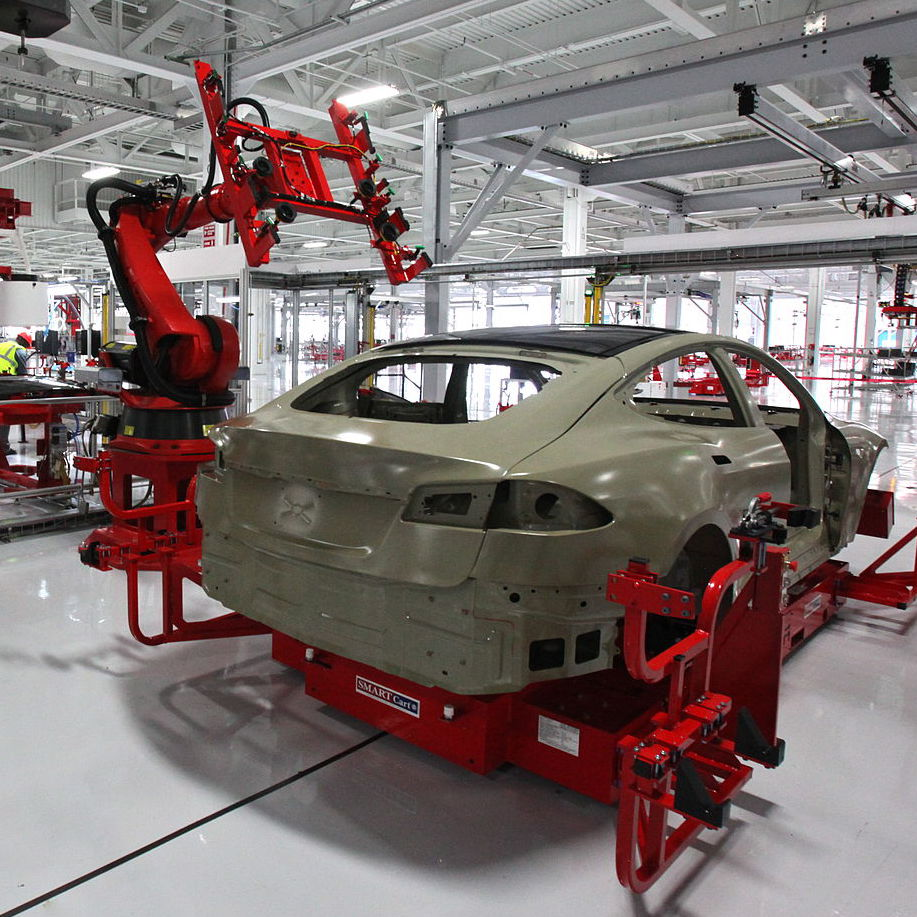
\includegraphics[width=0.32\linewidth]{figures/object_recognition/tesla.jpg}
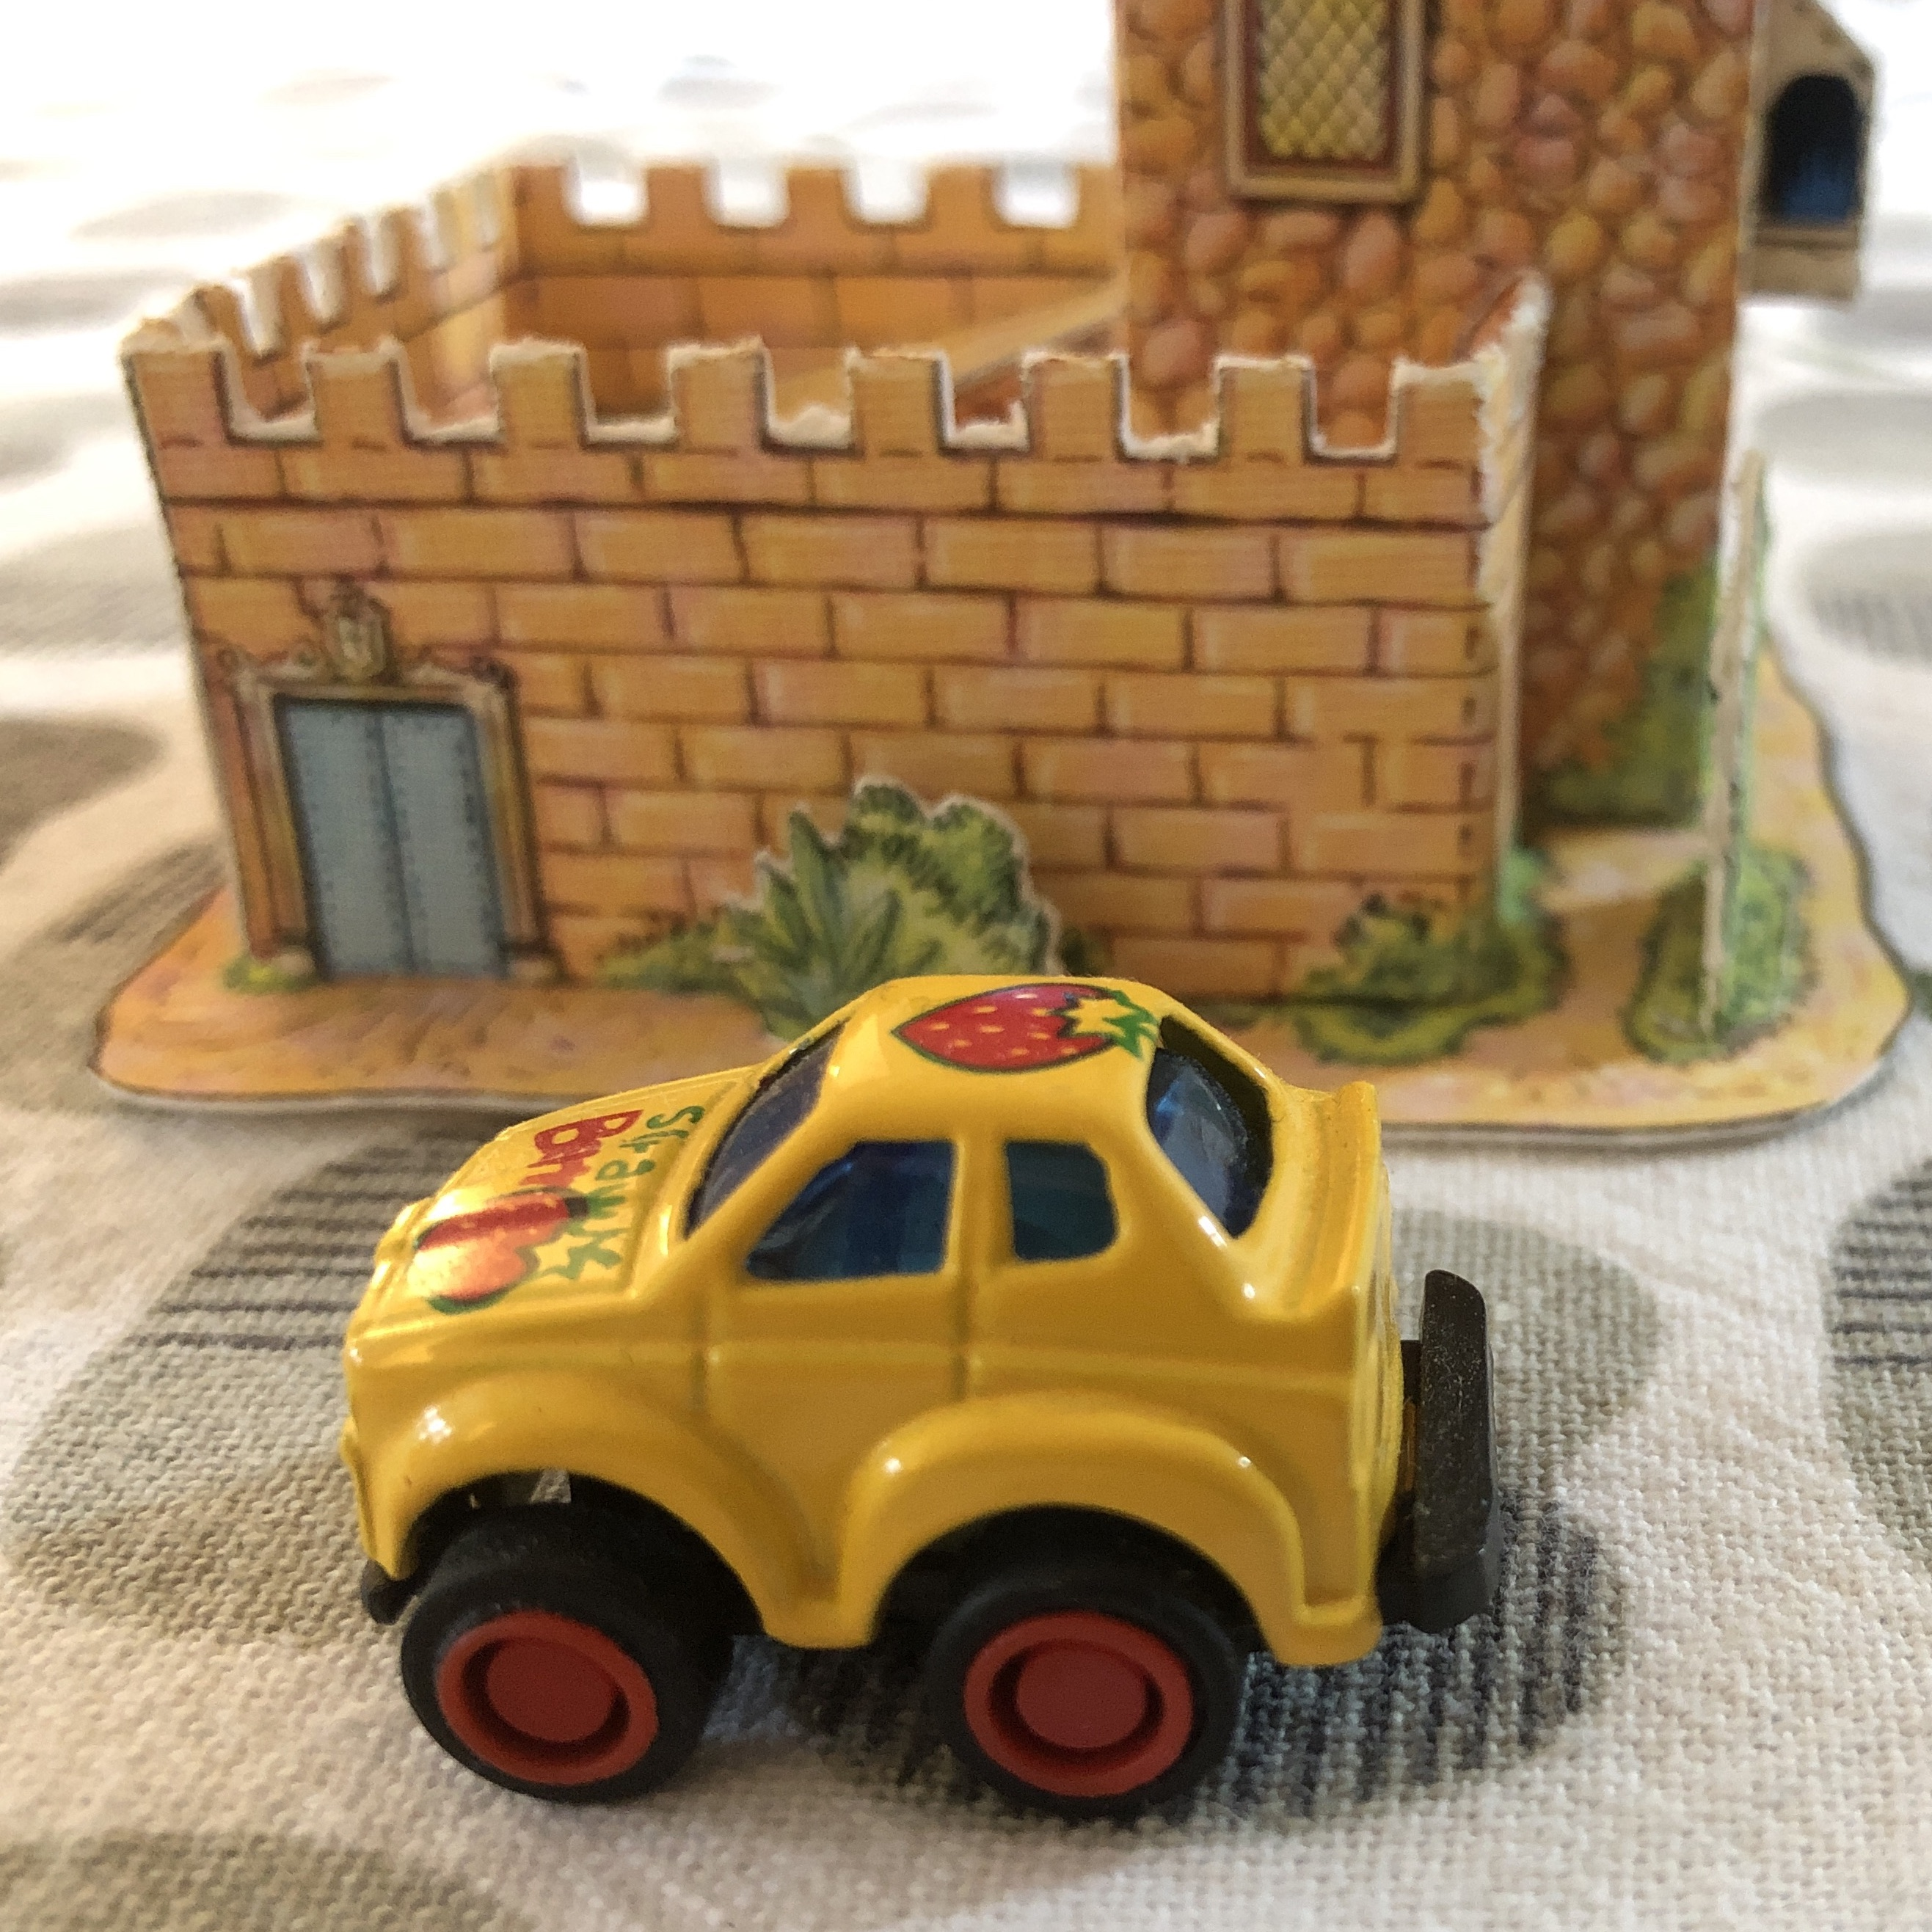
\includegraphics[width=0.32\linewidth]{figures/object_recognition/IMG_4467.jpeg}
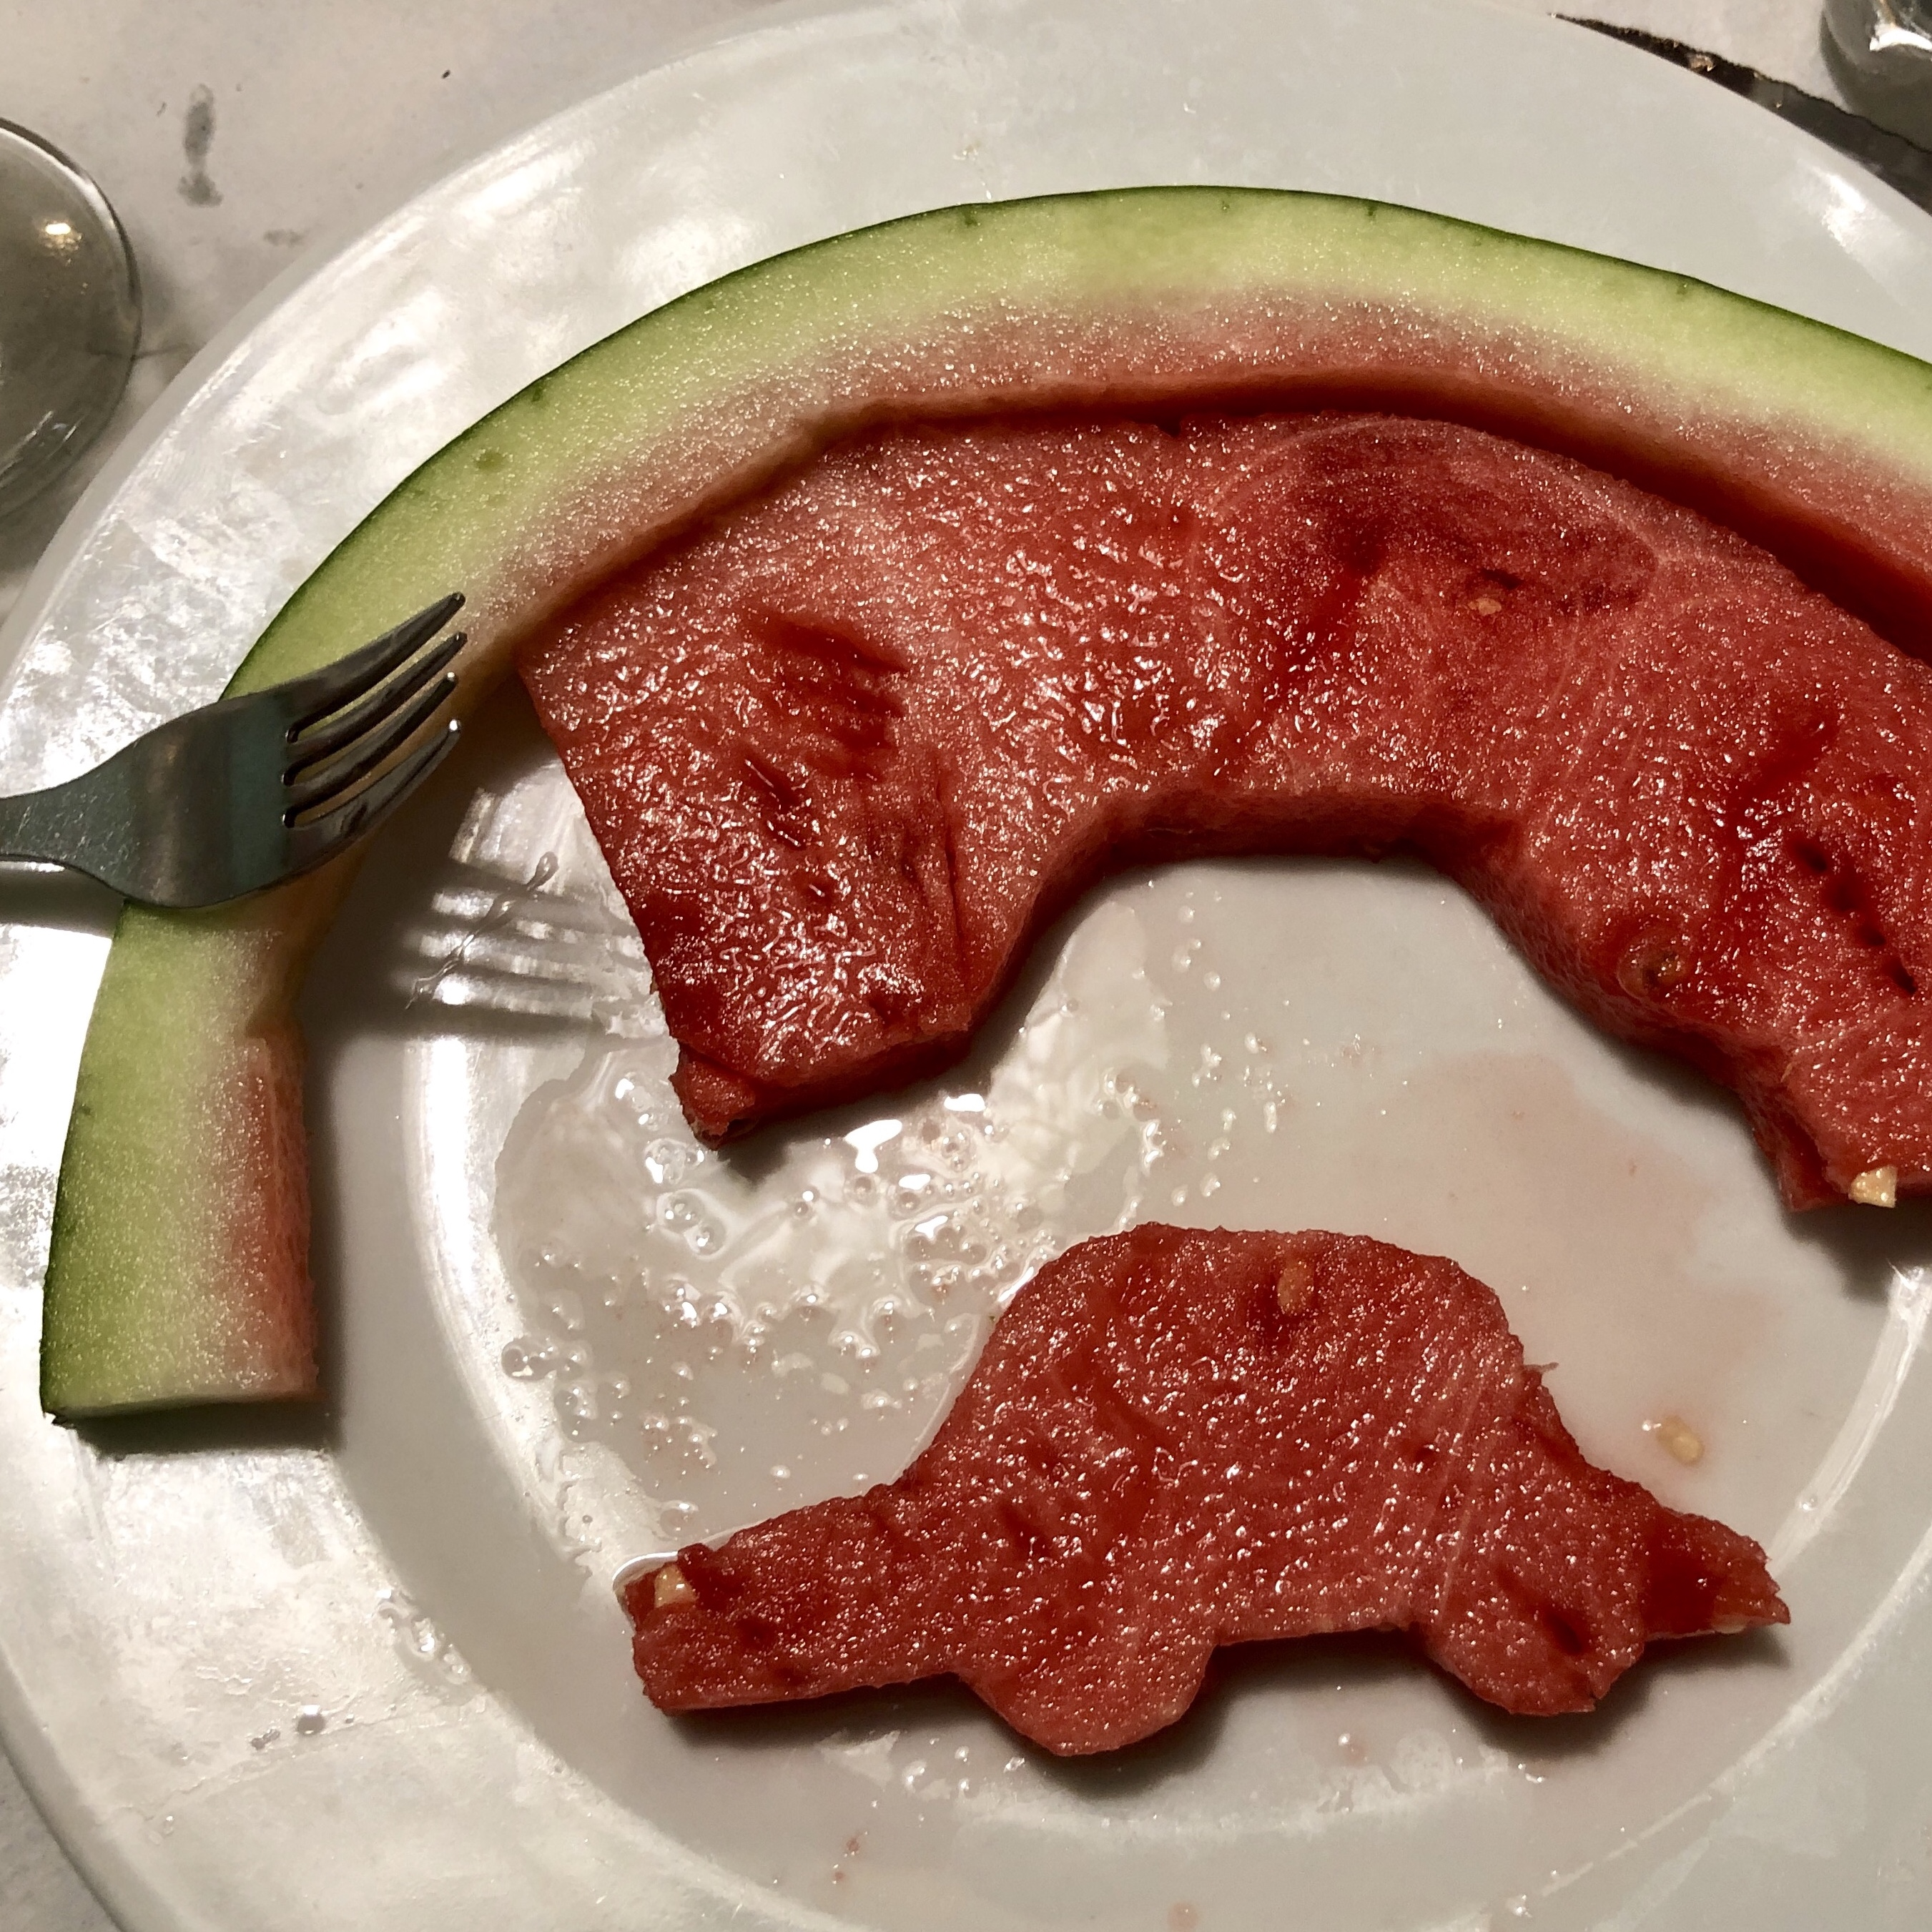
\includegraphics[width=0.32\linewidth]{figures/object_recognition/IMG_9325.jpeg}
}
\caption{Which of this images contains a car? A simple question that does not have a simple answer.}
\label{fig:whatisacar}
\end{figure}

What if there are multiple objects in the image?

What if the object is present in the scene but invisible in the image?


What if there are infinite classes?

In our formulation, $\hat {\bf y}$ is a vector of a fixed length. Therefore, we can only answer the question "is object class $c$ present in the image?" for a finite set of classes. What if we want to be able to answer an infinite set of questions?


Same or different
- deals with an infinite number of classes.

$y = f(x_1,x_2)$

\subsection{Localization}

Despite that the classifier has only been trained to detect the presence or absence of an object, it is possible that it has also learned to localize it in the image despite that it has not been explicitly trained to do so. 


Backpropagate, CAM

\section{Object detection and localization}

For many applications, saying that an object is present in the image is not enough. Suppose that you are building a visual system for an autonomous vehicle, if the system only tells the navigation system that there is a person in the image it will be insufficient to decide what to do.

Object localization consists in localizing where in the image is the object. There are many ways in which one can specify where the object is. The most traditional way of representing the object location is using a bounding box. 

FIGURE: show bounding boxes for some classes. 

\subsection{Formulation}

How you look at an object does not change the object (whether you see it or feel it, ...).  This induces translation and scale invariance. Let's build a system that has this property. 

Object localization 

function that maps the input image ${\bf x}$ into a list of bounding boxes $\hat {\bf b}_i$ and the associated classes to each bounding box encoded by a vector $\hat {\bf y}_i$.

This is usually done in four steps. In the first step, the algorithm produces a set of candidate bounding boxes. In the second step, we loop over all the candidate bounding boxes, we crop the image and resized to a canonical size, and then we apply an object classifier to classify the image as containing or not the object we are looking for. In the third step, we refine the bounding box for the crops that are classified as containing the object. And finally, in the fourth step, we discard overlapping detections likely to correspond to the same object to output only one bounding box for each instance present in the image. Each step can be implemented in several different ways giving rise to different approaches. 

\begin{algorithm}[h]
\label{object_localization}
\SetAlgoVlined
\DontPrintSemicolon
\caption{Object detection}
{\bf Input:} image;
{\bf Output:} trained models $f_{\theta^{N}}$ and $f_{\theta^{N+M}}$\;
Bounding box proposals\;

\For{\upshape $i= 1, \dots, N$}{
    Classification\;
    Bounding box refinement\;
}

Non-maximum suppression\;
\end{algorithm}



\begin{equation}
(\hat {\bf y}_i, \hat {\bf b}_i) = h({\bf x})
\end{equation}





As a regression problem. Input the object label and return its location:

$rect = f(x, y)$

Or as a classification problem: enter a location and return a label for the region:

$y = f(x, rect)$

Relate the definition to the measure of performance

Object detection: Search and classification
		Scanning window -> pyramids
		Selective search
		
\subsection{Localization loss}

\subsection{Evaluation}

Performance evaluation
		intersection over union. There are some  cool figures showing what IoU of 0.5 means, 0.7, 0.9, ... We could show this for bounding boxes and for segmentations  of dogs (or horses), showing examples of different segmentations and the associated measures. 
		precision-recall, ROC. Make a FIGURE  showing sets and what  each  measure represents. 
		average  precision  (AP), meanAP   (averaged across all categories)	
		
But why is object classification different from detection?

\subsection{Shortcomings}



The system is now penalized if it does not correctly localize the object. But it could still benefit from unintended correlations in the image. 

Overlapping boxes: bounding boxes can produce ambiguities when two objects overlap. It might not be clear which pixels belong to each object. 

Bounding boxes might be fine for certain applications or to describe some object classes. Bounding boxes are bad for objects that have long and thin structures (e.g. trees), or not well defined boundaries (the sky). Bounding boxes are also an insufficient object description if the task is robot manipulation. A robot will need a more detailed description of the pose and shape of an object to interact with it. 

Let's face it, localizing objects in images did not address most of the shortcomings present in the image classification formulation. In fact, it added a few more.
		
\section{Segmentation}

An object is something localized in space. There are other things that are not localized such as fog, light, ... Not everything is well described by a bounding box (stuff, wiry objects, ....)

Per pixel classification:

$y = f(x, n, m)$

or as more generic formulation: image in, $x(n,m)$, and segmentation out $y(n,m)$:

$y = f(x)$

Relate the definition to the measure of performance

Problems: 

- one label per pixel might not be appropriate. What happens with transparent objects (is a car outside of a window a car or a window?). 

- sometimes even humans can not segment correctly. If you see many chairs, can you tell who owns the legs?


\section{Summary}

Figure \ref{fig:pictorialsummary} shows a pictorial summary of the different methods we have seen in this chapter to represent objects in images. 

\begin{figure}
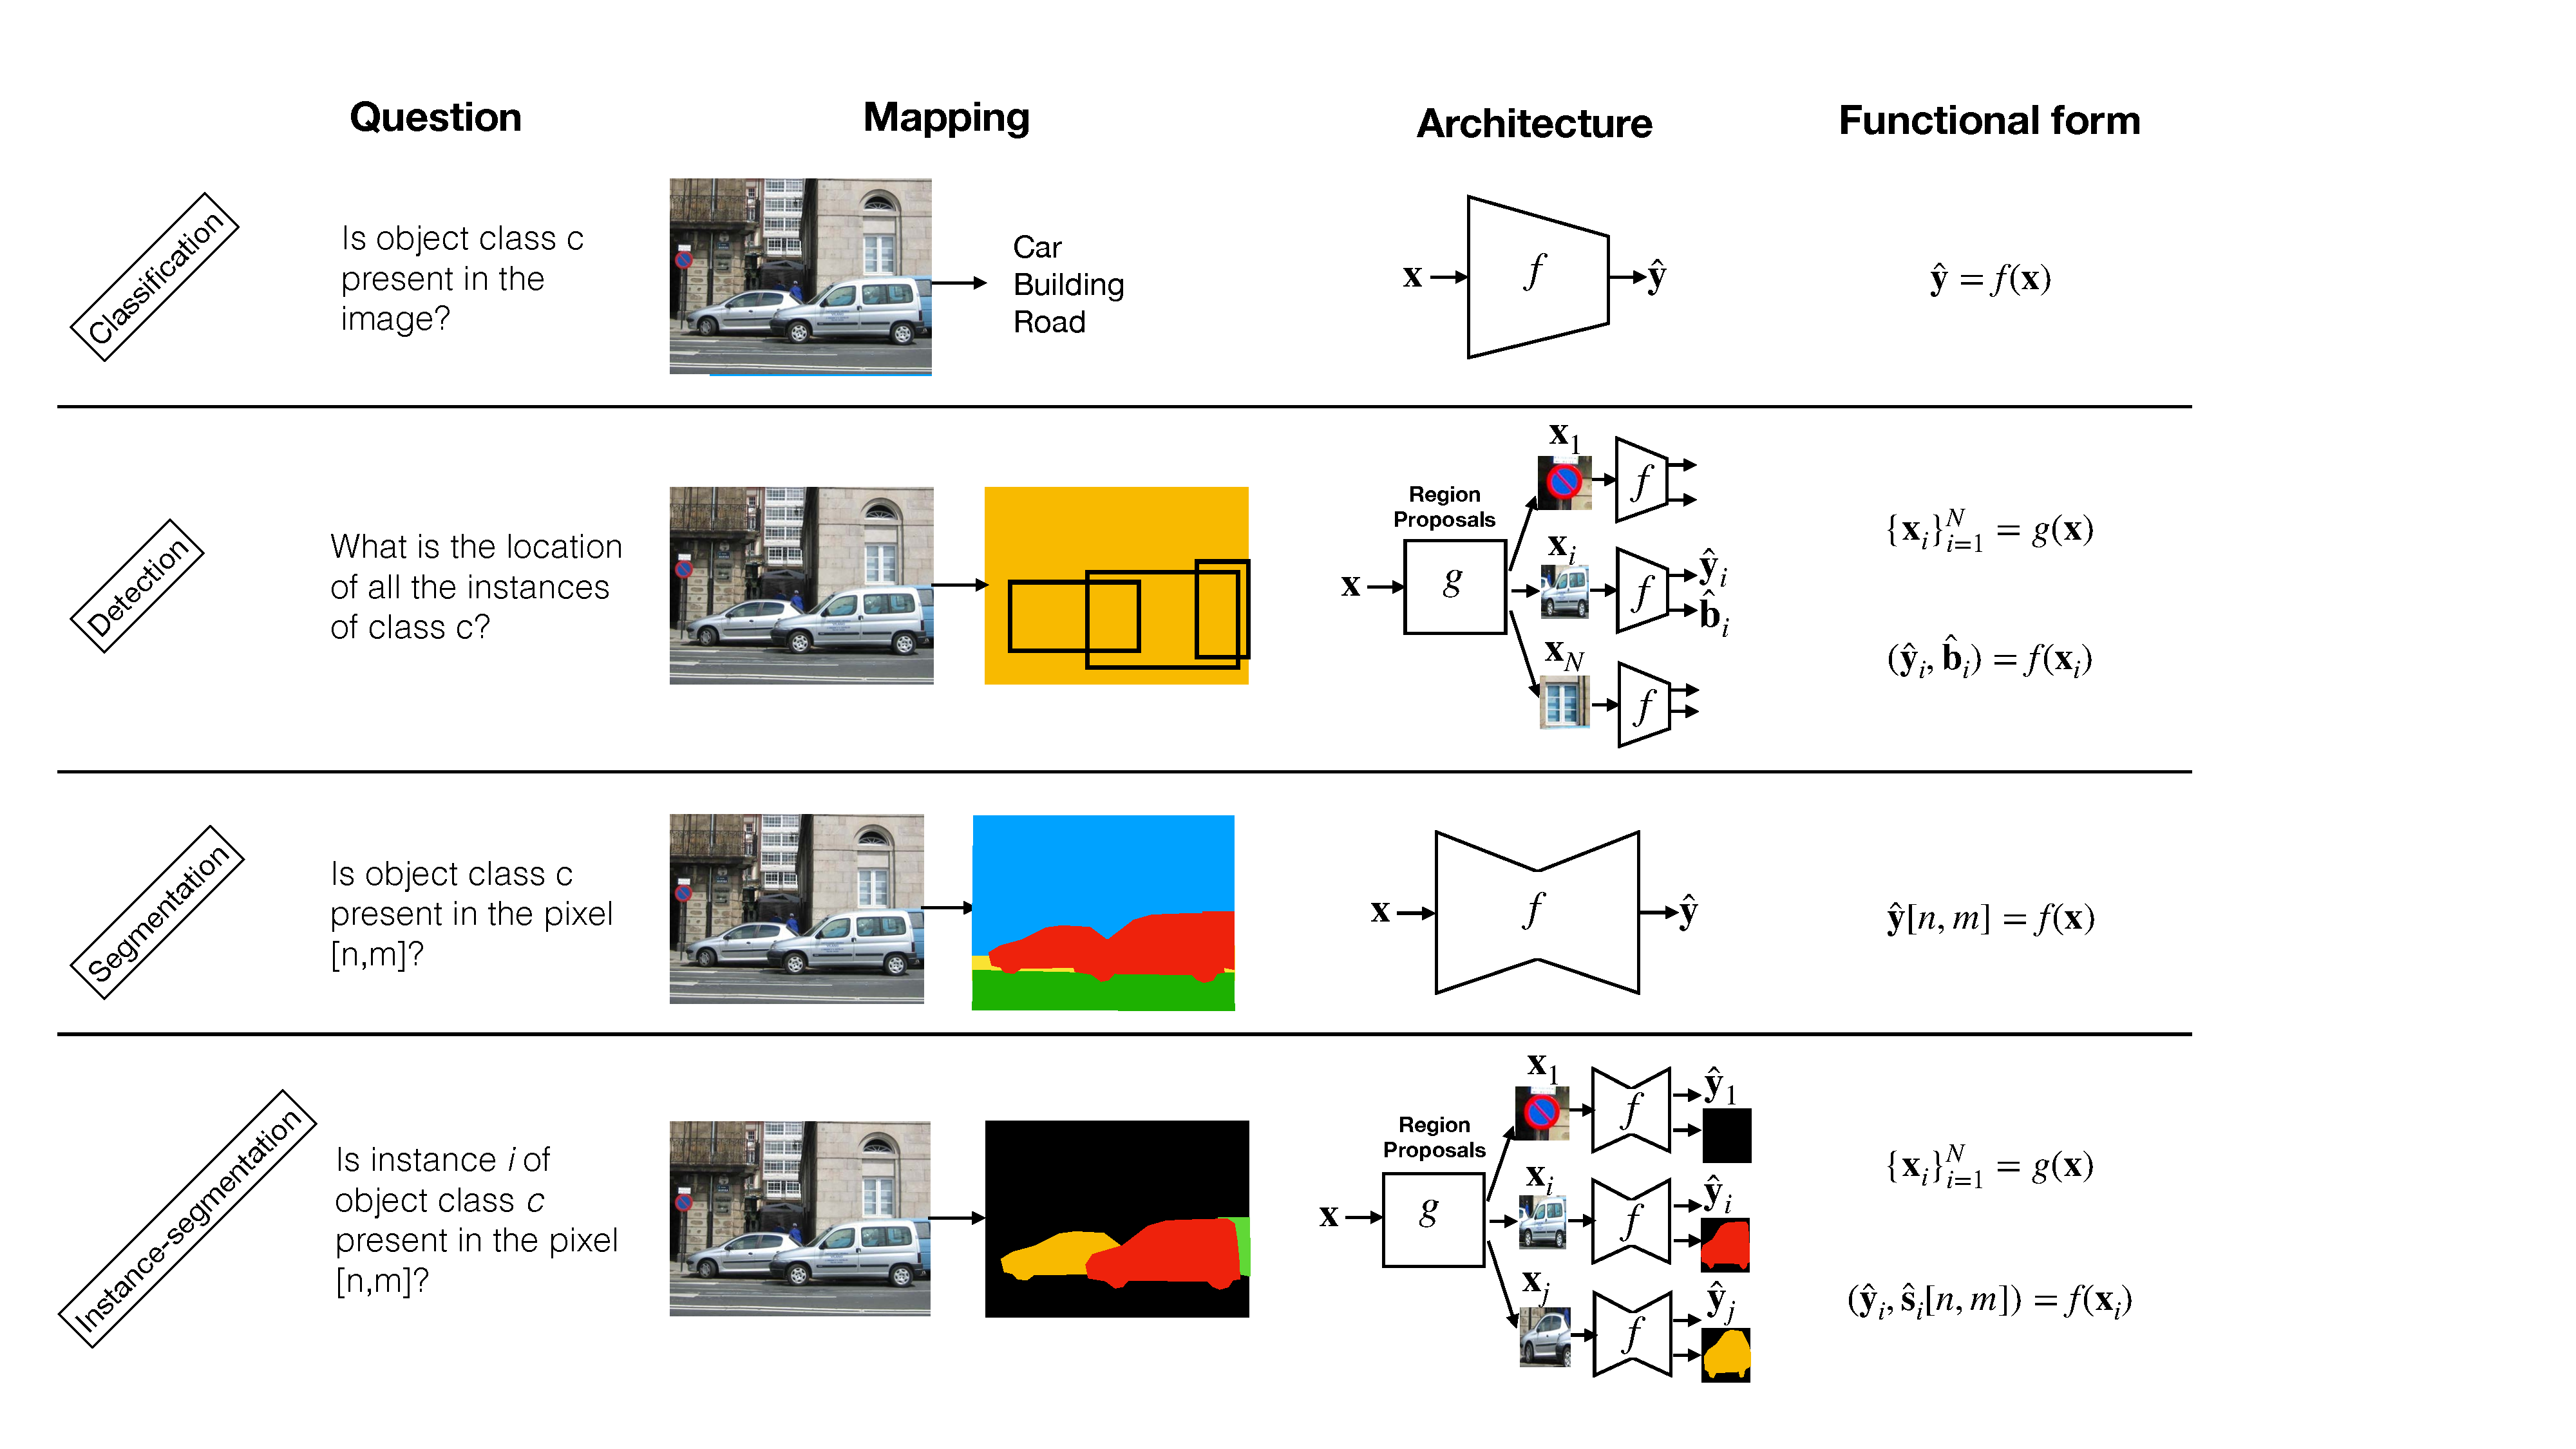
\includegraphics[width=1\linewidth]{figures/object_recognition/model_cards.pdf}
\caption{A family of object recognition definitions.}
\label{fig:pictorialsummary}
\end{figure}



\begin{comment}

\section{Layers}

the segmentation feels also a bit incomplete as it treats the output as a 2D image. But when we look at a scene, we also have labels for things that are occluded.

- handling multiple instances and occlusion
- a modal object completion

When formulated as a learning problem, the trick is to specify an output data structure that is learnable and satisfies our requirements. One example is, we could specify a label and output a binary segmentation mask and z ordering value.

$(s,z) = f(x,y)$

but then what happens if we have 

or w
\section{3D}
- meshes
- point clouds
- voxels
- volumetric models









% -> what is in forsyth book?

	
		
		
	Models
		blocks world
		3d compositional models
		geons
		deformable parts
		pictorial structures
		scene models
		context

		

			
	Similarity based models
		Prototypes
		Attributes
		Retrieval, similarity measures
		Retrieval by deformable alignment. 
		
	Semantic segmentation 
		Pixel classification: what is the generic formulation? 
	
	
	
	Levels of supervision - this go in another chapter? or maybe something very specific about this chapter. 
		
		
	Technical tricks
		Hard negative mining
		Non-maximal  supression

	Challenges
		Learning from little data
		Unsupervised object discovery
		
	Beyond recognition
		Attributes and affordances
		Shape base representations (deformable fields)
		Open world
		
%\chapter{3D scene understanding}


\end{comment}

